\section{Durchführung}

\begin{figure}[H]
  \centering
  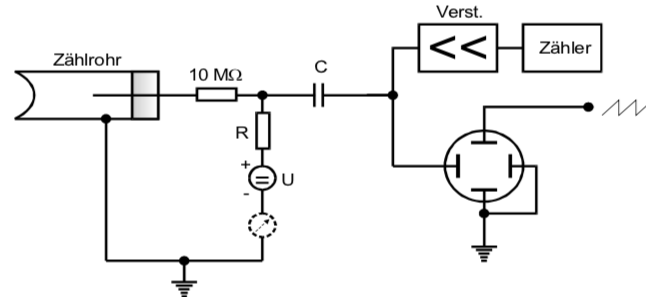
\includegraphics[width=\textwidth]{content/Aufbau.png}
  \caption{Versuchsaufbau \cite{1}.}
  \label{abb:5}
\end{figure}

In Abbildung \ref{abb:5} wird eine Skizze der Messapparatur gezeigt. Der Spannungsimpuls
wird durch den Widerstand R erzeugt und durch den Kondensator C ausgekoppelt. Daraufhin
wird der Impuls noch verstärkt und die Impulse können duch ein Zählgerät oder Oszilloskop
aufgezeichnet werden. Für alle Messreihen ist $\Delta t = \SI{60}{\second}$.

Als erstes wird die Charakteristik des Zählrohrs betrachtet. Dazu wird die Zählrate
in Abhängigkeit der Spannung gemessen. Es wird von \SI{300}{\volt} bis \SI{700}{\volt} gemessen.
Parallel dazu wird auch der Strom gemessen. Mit der folgenden Gleichung kann aus
dem gemessenen Strom auf die Ladungsmenge geschlossen werden.

\begin{equation}
  \overline{I} = \frac{\Delta Q}{\Delta t} Z
  \label{eq:1}
\end{equation}

Dabei sind Z die Teilchen die pro Zeit $\Delta t$ gemessen werden.

Daraufhin wird für drei verschiedene Spannungen die Totzeit untersucht. Dafür
werden die Messwerte auf einem Oszilloskop aufgetragen und erhalten ein Bild wie
in Abbildung \ref{abb:3}. Von dem Oszilloskop werden dann die Totzeit und Erholungszeit
abgelesen.

Als letzte wird die Totzeit durch die Zwei-Quellen-Methode bestimmt. Dazu wird zunächst
die Zählrate von Präparat 1 bestimmt, danach von Präparat 1 und 2 zusammen und als letztes
die von Präparat 2. Aufgrund der Totzeit wird $N_{1+2} < N_1 + N_2$ und mit der
Gleichung \ref{eq:2} lässt sich die Totzeit berechnen.

\begin{equation}
  T \approx \frac{N_1 + N_2 - N_{1+2}}{2 N_1 N_2}
  \label{eq:2}
\end{equation}
